\documentclass[crop,tikz]{standalone}% 'crop' is the default for v1.0, before it was 'preview'
\usepackage{physics}
\usetikzlibrary{positioning,shapes.geometric,decorations.pathreplacing,arrows.meta}
\begin{document}
\tikzset{meter/.append style={draw, inner sep=10, rectangle, font=\vphantom{A}, minimum width=30, line width=.8,
 path picture={\draw[black] ([shift={(.1,.3)}]path picture bounding box.south west) to[bend left=50] ([shift={(-.1,.3)}]path picture bounding box.south east);\draw[black,-latex] ([shift={(0,.1)}]path picture bounding box.south) -- ([shift={(.3,-.1)}]path picture bounding box.north);}}}

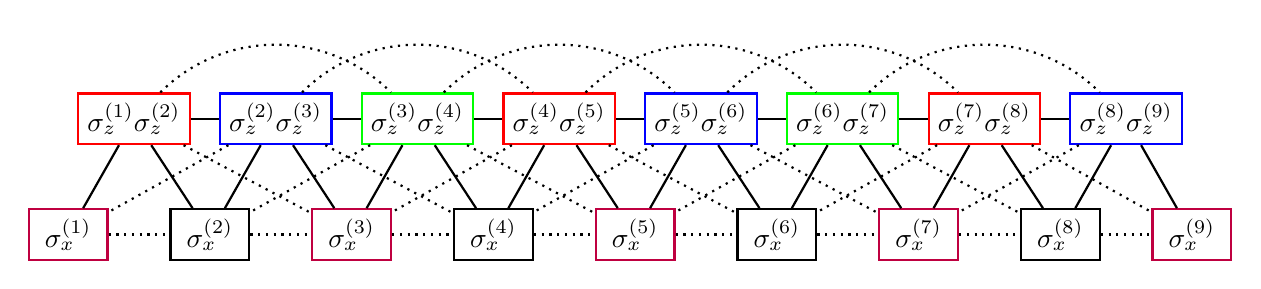
\begin{tikzpicture}[node distance={18mm}, thick, main/.style = {draw, rectangle,minimum width=1cm}
    ] 
\node[main, draw=red] (0)               {$\sigma_z^{(1)} \sigma_z^{(2)}$}; 
\node[main, draw=blue] (1) [right of=0] {$\sigma_z^{(2)} \sigma_z^{(3)}$};
\node[main, draw=green] (2) [right of=1] {$\sigma_z^{(3)} \sigma_z^{(4)}$};
\node[main, draw=red] (3) [right of=2] {$\sigma_z^{(4)} \sigma_z^{(5)}$};
\node[main, draw=blue] (4) [right of=3] {$\sigma_z^{(5)} \sigma_z^{(6)}$};
\node[main, draw=green] (5) [right of=4] {$\sigma_z^{(6)} \sigma_z^{(7)}$};
\node[main, draw=red] (6) [right of=5] {$\sigma_z^{(7)} \sigma_z^{(8)}$};
\node[main, draw=blue] (7) [right of=6] {$\sigma_z^{(8)} \sigma_z^{(9)}$};

\node[main] (8) [draw=purple,  below left=8mm and -4mm of 0] {$\sigma_x^{(1)}$};
\node[main] (9) [draw=black, below left=8mm and -4mm of 1] {$\sigma_x^{(2)}$};
\node[main] (10) [draw=purple, below left=8mm and -4mm of 2] {$\sigma_x^{(3)}$};
\node[main] (11) [draw=black, below left=8mm and -4mm of 3] {$\sigma_x^{(4)}$};
\node[main] (12) [draw=purple, below left=8mm and -4mm of 4] {$\sigma_x^{(5)}$};
\node[main] (13) [draw=black, below left=8mm and -4mm of 5] {$\sigma_x^{(6)}$};
\node[main] (14) [draw=purple, below left=8mm and -4mm of 6] {$\sigma_x^{(7)}$};
\node[main] (15) [draw=black, below left=8mm and -4mm of 7] {$\sigma_x^{(8)}$};
\node[main] (16) [draw=purple, below right=8mm and -4mm of 7] {$\sigma_x^{(9)}$};

\draw[-] (0) -- (1);
\draw[-] (1) -- (2);
\draw[-] (2) -- (3);
\draw[-] (3) -- (4);
\draw[-] (4) -- (5);
\draw[-] (5) -- (6);
\draw[-] (6) -- (7);

\draw[-] (0) -- (8);
\draw[-] (0) -- (9);
\draw[-] (1) -- (9);
\draw[-] (1) -- (10);
\draw[-] (2) -- (10);
\draw[-] (2) -- (11);
\draw[-] (3) -- (11);
\draw[-] (3) -- (12);
\draw[-] (4) -- (12);
\draw[-] (4) -- (13);
\draw[-] (5) -- (13);
\draw[-] (5) -- (14);
\draw[-] (6) -- (14);
\draw[-] (6) -- (15);
\draw[-] (7) -- (15);
\draw[-] (7) -- (16);

\draw[dotted] (0) to[out=45,in=135] (2);
\draw[dotted] (1) to[out=45,in=135] (3);
\draw[dotted] (2) to[out=45,in=135] (4);
\draw[dotted] (3) to[out=45,in=135] (5);
\draw[dotted] (4) to[out=45,in=135] (6);
\draw[dotted] (5) to[out=45,in=135] (7);

\draw[dotted] (8) -- (9);
\draw[dotted] (9) -- (10);
\draw[dotted] (10) -- (11);
\draw[dotted] (11) -- (12);
\draw[dotted] (12) -- (13);
\draw[dotted] (13) -- (14);
\draw[dotted] (14) -- (15);
\draw[dotted] (15) -- (16);

\draw[dotted] (1) -- (8);
\draw[dotted] (2) -- (9);
\draw[dotted] (3) -- (10);
\draw[dotted] (4) -- (11);
\draw[dotted] (5) -- (12);
\draw[dotted] (6) -- (13);
\draw[dotted] (7) -- (14);

\draw[dotted] (0) -- (10);
\draw[dotted] (1) -- (11);
\draw[dotted] (2) -- (12);
\draw[dotted] (3) -- (13);
\draw[dotted] (4) -- (14);
\draw[dotted] (5) -- (15);
\draw[dotted] (6) -- (16);

\end{tikzpicture} 
\end{document}
